% Celé zařízení je~rozděleno na~základní jednotku a~případné moduly, které zajistí nové herní možnosti.
%~Například může jít o~připojení úložného prostoru nebo zvukového modulu, který poskytne jak plnohodnotný zvukový výstup tak vstup.

%~\subsection{uživatelské požadavky}
Uživatelským požadavkem je~statické zařízení sloužící jako herní stanoviště.
Vyžaduje tedy mobilitu jen v~rámci transportu na~místo hry a~zpět, nikoliv v~rámci samotné hry.
Z~toho plynou požadavky na~velikost výsledného zařízení.

Zařízení bude mít dva světelné kruhy složené z~60 RGB LED.
Číslo 60~jsem zvolil, protože se~jedná o~dostatečně jemné dělení, aby se~daly dělat plynulé efekty.
Zároveň jde o~číslo, které koresponduje s~hodinovým ciferníkem a~stupnicí na~kompasu.
Jeden z~kruhů bude radiální a~druhý axiální.

Axiální kruh bude umístěn~na horní stranu zařízení a~bude sloužit primárně jako odezva pro hráče na~malou vzdálenost, např. při zadávání hesla.
Radiální kruh pak bude umístěn také v~horní části zařízení a~jeho účelem bude naopak signalizace na~delší vzdálenost.
Například může sloužit jako maják viditelný ve tmě i~na stovky metrů.


%TODO: dopsat a~vygenerovat ilustraci
Uvnitř axiálního světelného kruhu se~bude nacházet tzv. tlaková plocha. %\label{popisTlakovky1}
Jedná se~o~ovládací prvek podobný dotykové ploše s~tím rozdílem, že~je schopen měřit i~sílu, která na~něj působí.
% Tento prvek je~založen na~měření rezonanční frekvence snímacích LC~článků, nad kterými se~nachází tlaková plocha.
% Tlaková plocha je~vodivý objekt, ve~kterém se~cívkou LC~článku indukují vířivé proudy a~následně se~jimi indukují proudy zpět v~cívce LC~článku.
% Tím plocha ovlivňuje indukčnost cívky a~tedy i~rezonanční frekvenci LC~článku.
% Ovlivnění indukčnosti je~závislé na~vzdálenosti plochy od~cívky a~tedy i~na~síle, která na~plochu působí.
% Velikost síly, která na~plochu působí, totiž ovlivňuje její průhyb a~tedy i~vzdálenost od~cívky.
% Díky velkému rozlišení použitého čipu LDC1614 \cite{LDC1614} (28 bitů) je~možné měřit změny vzdálenosti v~řádu jednotek mikrometrů \cite{LDC1614LinearPositionSensing}.
% Tato metoda je~tedy schopna měřit vzdálenost plochy od~jednotlivých cívek, které jsou čtyři, a~plochu tak snímají na~čtyřech místech.
% Následně je~z~těchto hodnot možno dopočítat, jak je~plocha nakloněna a~tím určit, kde se~jí uživatel dotýká.
%~Protože je~zároveň možné určit i~sílu jakou uživatel při dotyku vyvinul, dostal tento systém jméno tlaková plocha. %~silová by~bývalo přesnější ale nějak mi~to nejde přes pysky

Aby bylo stanoviště reálně použitelné při hře, musí celou hru vydržet na~baterii.
Není ojedinělé, aby měla bojovka čtyři i~pět hodin bez přestávky.
Plus je~nutná časová rezerva a~čas na~nastavování.
Čas, který zařízení zvládne běžet z~baterie, silně závisí na~činnosti, ale nebylo by~zrovna ideální, kdyby baterie byla výrazně omezujícím faktorem.
Výdrž na~jedno nabití by~tedy měla být alespoň šest hodin.

Vzhledem k~plánu připojovat moduly je~nutné navrhnout mechanizmus připojení.
Bylo by~ideální, kdyby si~mohl uživatel říct, co~bude hrát za~hru, a~podle toho si~sám připojil moduly, které potřebuje.
Tomuto určitě nechci bránit, ale přímo to~podporovat nese~řadu problémů, jak ze~strany konektoru a~mechaniky, tak ze~strany softwaru.
Konektor by~totiž musel být ideálně beznástrojově rozpojitelný a~opětovně spojitelný a~přitom dostatečně pevný, aby se~zařízení mechanicky chovalo jako jeden celek.
Takový konektor je~ale poměrně složité vyrobit, tak aby byl spolehlivý, a~tak jde v~tuto chvíli jen o~možnost dalšího vývoje.
Ze softwarového pohledu jde pak o~problém, jak detekovat konkrétní modul a~hlavně o~otázku, jak se~chovat k~modulům, které jsou potenciálně záměnné.

% Dejme tomu, že~máme modul klávesnici a~modul dvířka.
% Dvířka jsou původně navržena primárně jako úložný prostor, díky detekci zavření je~lze ale použít i~jako pohodlná tlačítka a~v~některých hrách se~proto používají jen jako tlačítka.
% Potenciální modul klávesnice je~ovšem jen suma tlačítek.
% Při vytváření konkrétní hry na~míru modulům, které herní návrhář má~zrovna k~dispozici, je~tento problém nepodstatný, protože sám návrhář rozhodne, co~má jak být.
% Ale ve~chvíli, kdy jde o~hru navrženou pro jinou kombinaci modulů, nastává problém jak rozhodnout, zda se~dají dvířka použít místo klávesnice nebo ne~a~naopak.
% Abych se~všem těmto problémům alespoň prozatím vyhnul, rozhodl jsme se, že~doplnění či~výměna modulu půjde jen při servisním zásahu.
% Problém záměny modulů tak budu řešit tím, že~každá hra bude vytvořena jen pro konkrétní sadu modulů.

V~řadě případů je~užitečné mít možnost zvukové zpětné vazby.
Ideální by~bylo moci přehrávat libovolnou nahrávku, většinou ale stačí jednoduchý tón, řekněme jako potvrzení zadaného hesla.
Pro možnost přehrávání plnohodnotného zvuku bude proto sloužit samostatný modul a~v~základní jednotce, postačí jednoduchá sirénka.

Z~požadavků mi~vyplynulo zařízení, jehož možný vzhled je~nastíněn na~obrázku \ref{fig:AHS-nacrt}.
\begin{figure}[h]
    \centering
    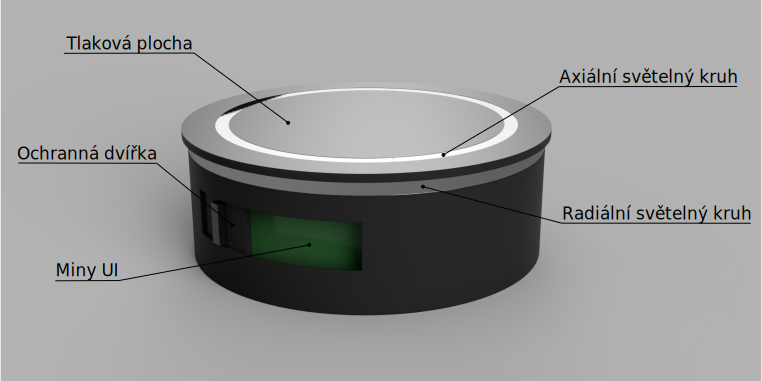
\includegraphics[width=\textwidth]{text/PraktickaCast/img/AHS-nacrt.png}
    \caption{Návrh vzhledu zařízení}
    \label{fig:AHS-nacrt}
\end{figure}

\newpage
\section{Elektronické systémy zařízení}

Elektronika bude~rozdělena na~dvě samostatné DPS.
Pujde o~hlavní desku, na~které bude umístěna většina elektroniky a~o~desku s~hlavním uživatelským rozhraním (LED deska).
Kompletní schéma a~topologie DPS je~k~vidění v~přílohách (schéma je~k vidění v~příloze \ref{AHS-sch} a~DPS v~příloze \ref{AHS-pcb}).

%~Původně jsem uvažoval ještě třetí desku, se~základním uživatelským rozhraním (mini~UI) pro usnadnění zajištění jisté míry voděodolnosti, ale nakonec jsem se~rozhodl spojit ji~s~hlavní deskou.

\subsection{LED deska}
Na LED desce budou umístěny oba světelné kruhy a~elektronika pro snímání tlakové plochy, tedy LDC1614 \cite{LDC1614} a~jeho snímací LC~články.
Právě snímaní tlakové plochy je~jeden z~hlavních důvodů oddělení této elektroniky na~samostatnou desku, zabere totiž na DPS velkou plochu.

Na LED desce se~tedy nachází:
\begin{itemize}
    \item Axiální LED kruh z~60 RGB LED WS2812B v~pouzdře \(3,5\)\;x\;\(2,8~mm\)
    \item Radiální LED kruh z~60 RGB LED WS2812B v~pouzdře \(3,5\)\;x\;\(2,8~mm\)
    \item LDC1614 se~čtyřmi snímacími LC~články pro snímání tlakové plochy 
    \item konektor na~propojení s~hlavní deskou
\end{itemize}

% Čip LDC1614 \cite{LDC1614} lze zaměnit za~LDC1314 \cite{LDC1314}, tyto čipy se~liší vlastně jen šířkou výstupního registru.
% Dalo by~se~tedy čekat snížení citlivosti při použití verze čipu LDC1314, není to~ale úplně pravda.
% Uživatel si~u~LDC1314 ale musí zvolit kompromis mezi rozsahem měření a~jeho citlivostí.
% Nastavení se~navíc dá~jednoduše měnit za~chodu, takže by~LDC1314 znamenalo nanejvýš trochu složitější program ale ne~nutně ztrátu citlivosti nebo rozsahu. 

\newpage
\subsection{Hlavní deska}

Řídícím mikrokontrolérem AHS bude ESP32-S3 (výběr je~rozebrán v~podsekci \ref{subs:vybermikrokontroléru}).
Na hlavní desce bude spolu s~mikrokontrolérem také zdroj poskytující správné napájení všech systémů zařízení.
Hlavní deska bude tedy zprostředkovávat několik napěťových větví.
V~neposlední řadě se zde bude nacházet základní uživatelské rozhraní v~podobě několika tlačítek, jednoduché RGB LED a sirénky.

Zdroj AHS je~tvořen dvěma LiIon články 18650 v~paralelním uspořádání.
Dva články volím, abych zajistil dostatečnou výdrž baterie a~abych využil volné místo v~zařízení.
Paralelní uspořádání jsem volil, aby nebyl nutný balancer při nabíjení, a~tedy abych zjednodušil zařízení.

Elektronika řeší i~nabíjení baterie, současně s~čímž realizuje i~ochranu proti podbití a~případnému přebití.
Aby nebylo možné softwarově baterii podvybít, má~AHS už~zmíněnou ochranu proti podvybití řešenou čistě hardwarově.
Tato ochrana tak celé zařízení vypne v~případě, že~dojde k~vybití baterie pod napětí \(2,8~V\).
Pochopitelně, software by~měl vybitou baterii zaznamenat mnohem dřív a~chovat se~podle toho, např. neumožnit spustit hru napětí na baterii \(3,0~V\).

Abych vyhověl napěťovým požadavkům všech použitých systémů, jsou na~hlavní desce tři různá napájecí napětí, která se~dál dělí do~šesti napájecích větví.
\begin{itemize}
    \item VCC, napětí baterie sloužící jako zdroj pro ostatní napájecí větve a~pro napájení komunikačního modulu. 
    \item Napětí \(3,3~V\) na~napájení logické části celého základního zařízení.
    \item Napětí \(5,0~V\) pro LED desku a~externí moduly a~napájení z~USB
    \begin{itemize}
        \item V-USB, z~USB-C konektoru pro nabíjení a~programování
        \item 5V-A, pro napájení modulu na~modulovém konektoru
        \item 5V-B, pro napájení LED kruhů
        \item 5V, jakožto zdroj pro větvě 5V-A a~5V-B 
    \end{itemize}
\end{itemize}
Napětí větví \(3,3~V\) je~tvořeno pomocí LDO.
Na vytvoření větve 5V~je ale potřeba spínaný zdroj.
Především proto, že napětí baterie, ze~které se~tato větev napájí, má~nižší napětí a~je jej tedy třeba transformovat na~napětí vyšší.
Navíc tento zdroj poskytuje do~systému proudy o~hodnotě až pět ampér a~bylo by~tedy vhodné použít spínaný zdroj i~v~případě vyššího vstupního napětí.
LDO by tak mělo malou efektivitu převodu a~především by~vytvářel nemalé množství odpadního tepla, se kterým by se zařízení muselo vypořádat.

Na hlavní desce je~také řada konektorů sloužících pro připojení ostatních systémů.
Jde o~konektory na:
\begin{itemize}
    \item propojení s~LED deskou,                % samostatný objekt
    \item externí moduly,                        % samostatný objekt
    \item USB-C (nabíjení a~programování AHS),   % externě definovaný objekt
    \item programátor,                           % samostatný objekt
    \item slot pro SD~kartu.
\end{itemize}
Do~konektorů by se také dal zařadit držák na~dva LiIon články 18650.

\subsection{Výběr mikrokontroléru \label{subs:vybermikrokontroléru}}
Požadavky na výbavu mikrokontroléru jsou:
\begin{itemize}
    \item WiFi,
    \item Bluetooth,
    \item alespoň 2~UARTy,
    \item alespoň 22~GPIO pinů,
    \item I2C,
    \item dostatečný výpočetní výkon pro hladký chod interpretru JavaScriptu nebo Pythonu.
\end{itemize}

Porovnání některých dostupných možností je~provedeno v~tab. \ref{tab:vybermikrokontroléru}.
\begin{table}[h]
    % \hspace{-20mm}
    \small
    \begin{tabular}{|l|l|l|l|l|c|}
        % \hline
        % mikrokontrolér                  ~&~Jádro         &~Počet GPIO pinů    & Počet UARTů  ~&~Počet I2C &~Wi-Fi a~Bluetooth                \\ \hline
        \hline
        \makecell{Mikro-\\kontrolér}    & Jádro         &~\makecell{Počet\\GPIO pinů} &~\makecell{Počet\\UARTů} &~\makecell{Počet\\I2C} &~\makecell{Wi-Fi a\\Bluetooth} \\
        \hline
        ESP32        \cite{ESP32}       &~2x Xtensa LX6 &~34    ~            & 3            ~&~2         &~\textcolor{green}{\checkmark}    \\ \hline
        ESP32-S3     \cite{ESP32S3}     &~2x~Xtensa LX7 &~45    ~            & 3            ~&~2         &~\textcolor{green}{\checkmark}    \\ \hline
        ESP32-C3     \cite{ESP32C3}     &~1x~RISC-V     &~16-22              & 2             &~1         &~\textcolor{green}{\checkmark}    \\ \hline
        ESP32-C6     \cite{ESP32C6}     &~1x~RISC-V     &~34    ~            & 3            ~&~2         &~\textcolor{green}{\checkmark}    \\ \hline
        PIC32MZ-W1  ~\cite{PIC32MZ}     &~DS60001192    & 62    ~            & 3            ~&~2         &~\textcolor{green}{\checkmark}    \\ \hline

        \textcolor{red}{nRF7000      \cite{nRF7000}}      &~-             &~\textcolor{red}{13}& \textcolor{red}{0} &~\textcolor{red}{0}    & \textcolor{green}{\checkmark}    \\ \hline
        \textcolor{red}{RTL8710      \cite{RTL8710}}      &~ARM Cortex-M3 &~\textcolor{red}{17}& \textcolor{red}{1} &~3                     &~\textcolor{green}{\checkmark}    \\ \hline
        \textcolor{red}{RTL8721DM    \cite{RTL8721DM}}    & -            ~&~\textcolor{red}{17}& 3                  & 2                    ~&~\textcolor{green}{\checkmark}    \\ \hline
        \textcolor{red}{STM32WB55    \cite{STM32WB55}}    & ARM Cortex-M4 &~37    ~            & \textcolor{red}{1} &~2                     &~\textcolor{red}{$\times$}        \\ \hline
        \textcolor{red}{MSP430BT5190 \cite{MSP430BT5190}} &~-             &~32                 &~4                 ~&~4~                   ~&~\textcolor{red}{$\times$}        \\ \hline
    \end{tabular}
    \caption{Dostupné vyhovující mikrokontroléry}
    \label{tab:vybermikrokontroléru}
\end{table}

Abych nemusel návrh komplikovat anténou, použil jsem v~návrhu mikrokontrolér na~modulu, který má~anténu integrovanou, a~navíc integruje i~flash paměť. 
Protože už~tyto moduly interně používají některé GPIO, klesne množství, které mohu využít.

\begin{table}[h]
    \centering
    \begin{tabular}{|l|l|l|l|l|}
        \hline
        mikrokontrolér                  & Počet GPIO pinů    & vyhovuje?                     \\ \hline
        ESP32-WROOM     \cite{ESP32}    & 26                 & \textcolor{green}{\checkmark} \\ \hline
        ESP32-S3-WROOM  \cite{ESP32S3}  & 36                 & \textcolor{green}{\checkmark} \\ \hline
        ESP32-C3-WROOM  \cite{ESP32C3}  & 15                 & \textcolor{red}{$\times$}     \\ \hline
        ESP32-C6-WROOM  \cite{ESP32C6}  & 23                 & \textcolor{green}{\checkmark} \\ \hline
        WFI32E01PC      \cite{PIC32MZ}  & 37                 & \textcolor{green}{\checkmark} \\ \hline
    \end{tabular}
    \caption{Moduly s~mikrokontroléry}
    \label{tab:ModulySmikrokontroléry}
\end{table}

Jedním z~požadavků na~zařízení je~dostatečný výpočetní výkon pro hladký chod interpretu JavaScriptu nebo Pythonu.
Výpočetní výkon se~porovnává poněkud složitěji, protože se~nejedná tak úplně o~jeden parametr.
V~tomto případě je~ale vhodné prozkoumat i~dostupnost interpretu pro daný mikrokontrolér.
Pro ESP32 a~ESP32-S3 je~dostupný JavaScriptový interpret Jaculus \cite{Jaculus} i~interpret jazyka Python MicroPython \cite{MicroPythonESP32S3} \cite{MicroPythonESP32}.
Pro PIC32MZ-W1 a~ESP32-C6 je~dostupný pouze interpret jazyka Python MicroPython \cite{MicroPythonPIC32MZ-W1} \cite{MicroPythonESP32C6}. %interpret JavaScriptu jsem však nenašel.
ESP32 a~ESP32-S3 tak poskytuje výhodu v~možnosti volby skriptovacího jazyka.
ESP32-S3 má~oproti starší verzi ESP32 výkonnější jádro a~interpret JavaScriptu, resp. Pythonu, na~něm tak běží o~něco plynuleji.

Další výhodou ESP32-S3 oproti PIC32MZ-W1 je~jeho cena, která se~pohybuje okolo 4~USD \cite{JSC-ESP32-S3}.
Zatímco PIC32MZ-W1 je~u~JLCPCB za~13.65~USD \cite{JSC-WFI32}.
Navíc u~firmy JLCPCB, kde plánuji elektroniku vyrábět, sice je~PIC32MZ-W1 v~nabídce, ale není na~skladě \cite{JSC-WFI32}, zatímco u~ESP32-S3 bylo v~době návrhu dostupných hned 19~variant \cite{JSC-ESP32-S3}.

V~mém případě má~ESP32-S3 ještě jednu podstatnou výhodu, a~tou je~fakt, že~s~rodinou mikrokontrolérů ESP32 mám dlouholeté zkušenosti.
Z~těchto důvodů jsem se~rozhodl pro ESP32-S3.

\subsection{Tlaková plocha \label{popisTlakovky2}}
Tlaková plocha je~založena na~měření indukčnosti čtyř cívek.
Tyto cívky jsou použity spolu s~paralelně řazeným kondenzátorem, aby dohromady tvořily rezonanční LC~článek.
Zároveň jsou cívky vytvořeny jako reliéf v~mědi DPS, aby jimi vytvořené magnetické pole sahalo mimo ně~a~dalo se~tak použít pro ovlivnění jejich vlastností.

V~objektu vloženém do~proměnného magnetického pole vytvářeného cívkou se~vytváří vířivé proudy, které následně tvoří magnetické pole ve~směru opačném k~poli vytvořenému cívkou.
Magnetické pole vzniklé z~vířivých proudů tak indukuje další proudy zpět v~cívce, čímž snižuje její zdánlivou indukčnost.
Ve výsledku tak objekt v~magnetickém poli cívky ovlivňuje její indukčnost.
Velikost indukovaných vířivých proudů a~tedy i~míra ovlivnění indukčnosti cívky, je~závislá na~vodivosti daného objektu (terčíku), na~jeho rozměrech a~na jeho poloze vůči cívce.
V~případě pohybu terčíku, pouze ve~směru kolmém k~ploše DPS s~vytvořenou cívkou, se~tak převádí vzdálenost terčíku a~DPS na~indukčnost cívky.
Vizualizace popsaného mechanizmu sa nachází na obr. \ref{fig:pryncip-LDC}.

\begin{figure}[h!]
    \centering
    \includegraphics[width=\textwidth]{text/PraktickaCast/img/civka_tercik_ilustrace.png}
    \caption{Princip převodu vzdálenosti na~indukčnost}
    \label{fig:pryncip-LDC}
\end{figure}

Protože pro indukci vířivých proudů v~terčíku musí být magnetické pole cívky proměnné, musí být i~proud cívkou proměnný a~tedy i~napětí na~celém LC~článku.
V~případě použití čipu LDC1614 je~tedy LC~článek chvíli buzen nastaveným proudem, dokud nedosáhne nastavené napěťové amplitudy.
Následně přejde do~stavu měření, ve~kterém změří rezonanční frekvenci LC~článku porovnáváním s referenčním oscilátorem.
LDC1614 má interní oscilátor s~frekvencí \(40\)~{\itshape MHz}, ale např. v~aplikacích náročných na~přesnost je~možné připojit oscilátor externí. 
V~případě využití více kanálů následně přepne na~další kanál a~opakuje stejný postup \cite{LDC1614}.

Princip tlakové plochy tedy spočívá ve~snímání vzdálenosti terčíku, se~kterým přichází do~kontaktu uživatel, čtyřmi snímacími cívkami na~LED desce.
Princip uspořádání je~zobrazen na~obrázku č.\ref{fig:nastin-tlakovky}.

Kromě katalogových listů čipu LDC1614 jsem vycházel i~z~informací uvedených v~aplikační poznámce firmy Texas Instruments \cite{LDC1614SensorDesign} a~ze skript předmětu Mikrosenzory a mikroelektromechanické systémy \cite{SkriptaMMS}

\begin{figure}[h!]
    \centering
    \includegraphics[width=\textwidth]{text/PraktickaCast/img/naklonena-tlakovka.png}
    \caption{Nástin principu snímání tlakové plochy}
    \label{fig:nastin-tlakovky}
\end{figure}

\subsection{Propojení hlavní desky a~LED desky}
Mezi hlavní deskou a~LED deskou je~třeba převést napájení a~několik signálů.
LED deska vyžaduje na~konektoru přítomnost dvou napájecích větví, \(5~V\) pro světelné kruhy a~\(3.3~V\) pro snímání tlakové plochy.
Protože do~RGB diod může téct proud až~\(5~A\) a~může být zároveň i~rychle spínaný, považuji za~rozumné oddělit napájecím větvím zem, abych omezil průnik rušení z~diod do~snímání tlakové plochy.
Oddělení je~tedy provedeno už~na konektoru hlavní desky a~už~v~kabelu jsou tedy větve vedeny samostatně.

Na samotné propojení jsem se~rozhodl použít FFC kabel s~roztečí \(0.5~mm\), pro jeho rozměry a~cenovou dostupnost.
Jedním vodičem takovéhoto kabelu lze vést proud maximálně \(0.4~A\) \cite{FFC-konektor}.
Protože ale potřebuji dodat proud až~\(5~A\), použiji \(13\) vodičů vedle sebe pro jednu cestu, jakožto nejmenší počet, který přenese~požadovaný proud v~rámci daných mezí.

Mimo napájení je~tímto propojením veden i~signál s~daty pro světelné kruhy a~I2C sběrnice se~signálem přerušení pro připojení čipu LDC1614 \cite{LDC1614}.
Výsledný počet vodičů v~kabelu je~tedy \(2 \cdot 13\) pro napájení, \(1\) pro data k~LED kruhům, dále \(2\) pro I2C, \(1\) pro signál přerušením a~nakonec \(2\) pro napájení snímání tlakové plochy.
Dohromady tedy kabel potřebuje \(32\) vodičů. 

Vzhledem k~počtu potřebných vodičů jsem se~rozhodl použít běžný FFC kabel se~40 kontakty s~tím, že~zbylé kontakty se~mohou hodit v~budoucnu.

\subsection{Modulový konektor \label{sec:ModulovyKonektor}}
Modulovým konektorem je~vedeno \(5~V\) jako napájení pro moduly a~komunikační sběrnice se~signálem přerušení pro komunikaci.

Nad volbou komunikační sběrnice jsem strávil značné množství času.
Původně jsem uvažoval o~využití RS485 jakožto odolné sběrnice, u~které by~v~případě potřeby nemusel být problém ani delší kabel.
RS485 má~ale nevýhodu v~tom, že~potřebuje dodatečný hardware, kterému bych se~hlavně na~modulech rád vyhnul.
Obdobný problém nastal u~CANu a~USB.
USB by~navíc mělo výhodu kompatibility s~velkým množstvím hotových zařízení.

V~první úvaze o~využití UARTu jsem jej zavrhl kvůli potenciální náročnosti na~přeposílání dat mezi moduly.
Při standardním použití bych totiž moduly řadil do~řetězu za~sebe.
Prvnímu modulu by~tak chodila data pro všechny ostatní moduly a~musel by~je přeposílat dál, což by~mohlo stát nezanedbatelné množství procesorového času.
%~TODO: nová linka, duvody, obhajoba

V~jisté chvíli jsem ale narazil na~nestandardní komunikaci pomocí UARTu implementované v~projektu Servio \cite{Servio}.
Tato implementace používá UART jako sběrnici.
Namísto standardního použití pro komunikace jeden-s-jedním tak může komunikovat jeden-s-více.
Na tomto řešení je~výhodné, že~nevyžaduje žádný dodatečný hardware a~prakticky každý dnešní mikrokontrolér je~možné k~této sběrnici velmi snadno připojit.

Ve srovnání s~RS485 je~sice mnohem méně odolná proti rušení, ale uvnitř zařízení nebude linka vedena na~příliš velkou vzdálenost.
Komunikace na~delším kabelu je~pak jednoduše nahraditelná bezdrátovou komunikací a~není tak potřebné, aby to~tato sběrnice v~základu podporovala.
% Navíc v~případě potřeby delšího kabelu je~možné navrhnout externí modul, který z~této sběrnice velmi jednoduše udělá RS485 pro externí využití.
% Alternativně by~se~pro komunikaci na~delším kabelu dalo použít USB, které je~společně s~nabíjením přivedeno na~USB-C.

Všechny moduly jsou připojeny na~jeden RX~pin AHS.
Proto musí firmware AHS zajistit, aby dva moduly nevysílaly současně.
Aby se~zabránilo možným zkratům, má~jako ochranu každý modul své piny UARTu připojeny přes rezistor \(180~\Omega\).
Pin~přerušení má na modulech naproti tomu jen schopnost signál přizemnit a~na straně hlavního zařízení je~dráha připojena přes rezistor k~napětí \(3,3~V\).
Abych alespoň trochu zvýšil odolnost linky proti rušení, přidám na~přijímací stranu pull-up rezistor.
Cílem je~zvýšení komunikačního proudu, aby se~případný proud vyvolaný rušením neprojevil.
V~neposlední řadě mají všechny piny na~konektoru ESD ochranu \cite{TPD4E02B04}.

\subsection{Konektor programátoru}
Zařízení se~dá jednoduše programovat přes USB-C, tento kanál je~ale možné softwarově narušit a~pro takové případy je~tu konektor na~programátor.
Jde o~šest plošek, na~které se~programátor připojuje pomocí pružinkových kontaktů.
Programátor sice obsahuje jen jednoduchou elektroniku, která by~mohla být i~přímo v~elektronice AHS, ale ve~většině případů by~byla zbytečná.
Ve chvíli, kdy by~byla potřeba, je~stejně nutná odborná obsluha a~pro tu~není problém použít externí programátor.

\subsection{USB-C}
USB-C je~použito pro nabíjení a~pohodlnější programování zařízení bez potřeby programátoru.

USB-C v~základu neposkytuje žádné napájecí napětí, protože je~navrženo k~obousměrnému provozu a může napájení jak poskytovat, tak spotřebovávat.
% Asi nejjednodušší zpusob jak požádat zdroj o~napájení je~dva rezistory s~hodnotou \(5.1~k\Omega\), přes které se~připojí signály \(CC1\) a~\(CC2\) k~zemi.
Asi nejjednodušší způsob jak požádat zdroj o~napájení, je~připojit dráhy {\it CC1} a~{\it CC2} k zemi přes rezistory o~hodnotě \(5.1~k\Omega\).
Takto zařízení dostane napětí \(5~V\) s~omezením proudu do~\(0.5~A\), tedy výkon \(2.5~W\).
V~tuto chvíli by~se~zařízení už~mohlo nabíjet, výkonem \(2.5~W\) by~se~ale nabíjelo velmi pomalu.
Proto jsem implementoval další systém, který má~za úkol zvýšit nabíjecí výkon a~tak zrychlit nabíjení.
Čip BQ25895M \cite{BQ25895} slouží primárně pro řízení nabíjení, ale zároveň se~stará o~komunikaci se~zdrojem a~zprostředkovává tak vyšší nabíjecí proud.
Velikost nabíjecího proudu se~navíc dá~v~případě potřeby nastavit přes I2C sběrnici z~ESP32-S3.

\subsection{Správa zapínání}
Zařízení je~vybaveno obvodem umožnujícím vypnutí jak uživatelské, tak programové a~v~případě hrozícího podbití i~automaticky.
Tento obvod zároveň kontroluje i~potenciální přebití baterie a~v~takovém případě odpojuje napájení nabíječky.

Původní verze správy zapínání je~vidět na~obr. \ref{fig:stary_PoverManager} (zapojení zapínacího tlačítka je~zjednodušeno, protože jeho zapojení je~složitější z~důvodu jeho čtení z~procesoru).

Na úvod popisu funkce je~vhodné říct, že~rezistor \(R_{5}\) slouží pro definici napětí na~\(G\) tranzistoru \(Q_{2}\) ve~chvíli vypnuté větve {\it 3V3} a~má~dostatečně velký odpor, aby se~při ostatních úvahách dal zanedbat.
Hlavní spínač je~PMOS tranzistor \(Q_{p1}\), který je~řízený NMOS tranzistory \(Q_{1}\) a~\(Q_{2}\).
Obvod \(U_{1}\) kontroluje stav baterie a~v~případě nízkého napětí na~dráze {\it Baterie} předpokládá, že~došlo k~limitnímu vybití baterie a~připojí na~vývod {\it OD}~(Over Discharge) \(0~V\) \cite{SL8261}.
To znamená zavřený tranzistor \(Q_{1}\), což znamená, že~se~rozepne i~tranzistor \(Q_{P1}\), protože se~jeho elektroda \(G\) vybije skrz rezistor \(R_{2}\).
Pokud je~baterie naopak nabita dostatečně, je~na vývod \(OD\)~obvodu \(U_{1}\) přivedeno jeho napájecí napětí \cite{SL8261}, v~našem případě tedy napětí baterie, které je~tak přivedeno na~\(G\) tranzistoru \(Q_{1}\).
Tranzistor \(Q_{1}\) je~tak otevřený, což znamená, že~zařízení má~povolení k~zapnutí. 
Když v~tuto chvíli dojde ke~stisku zapínacího tlačítka, přivede se~\(0~V\) na~\(G\) tranzistoru \(Q_{p1}\) a~dojde k~jeho otevření.
Následně naběhne napájecí větev {\it 3V3}, na~které bylo do~té doby \(0~V\).
Přes rezistor \(R_{4}\) se~tak přivede napětí {\it 3V3} na~\(G\) tranzistoru \(Q_{2}\) a~dojde k~jeho otevření.
Po otevření tranzistoru \(Q_{2}\) je~tranzistor \(Q_{p1}\) trvale otevřen a~zařízení je~tak zapnuto.

Následné vypnutí je~možné třemi cestami:
\begin{itemize}
    \item vybití baterie,
    \item povel z~procesoru,
    \item uživatelské tlačítko (v~pozdější verzi bylo odstraněno).
\end{itemize}

Ve chvíli, kdy dojde k~vybití baterie, zareaguje na~to obvod \(U_{1}\) rozepnutím tranzistoru \(Q_{1}\), čímž pomocí rezistoru \(R_{2}\) rozepne i~tranzistor \(Q_{p1}\) a~zařízení se~tak vypne.

Když procesor dostane příkaz k~vypnutí zařízení, stáhne dráhu {\it OFF} k~zemi, čímž vybije kapacitu \(C_{2}\) a~současně kapacitu \(G\) tranzistoru \(Q_{2}\), čímž dojde k~rozepnutí tranzistoru \(Q_{2}\).
Následně dojde k~rozepnutí tranzistoru \(Q_{p1}\) a~poklesu napětí na~napájecí větvi {\it 3V3}.
Z~této větve běží mimo jiné i~procesor a~není tedy jisté, že~udrží dráhu {\it OFF} na~napětí \(0~V\) až~do konce vypínání.
To je~důvodem přítomnosti kondenzátoru \(C_{2}\), který sice zpomalí reakci obvodu na~příkaz k~vypnutí, ale následně zajistí, že~se~obvod skutečně vypne.
Stisk tlačítka {\it OFF} má~reakci obdobnou. 

\begin{figure}[h!]
    \centering
    \includegraphics[width=\textwidth]{text/PraktickaCast/img/stary_power_manager.png}
    \caption{Původní verze správy zapínání}
    \label{fig:stary_PoverManager}
\end{figure}

Tato varianta však měla jeden problém způsobený absencí hystereze u~čipu kontrolující napětí baterie SL8261 \cite{SL8261}.
Ve chvíli, kdy se~baterie dostane do~stavu, kdy je~potřeba ji~odpojit, kontrola ji~skutečně odpojí.
To by~bylo správně, jenže z~baterie v~tu~chvíli pořád teče proud, který způsobuje úbytek jejího napětí.
Při přerušení proudu z~baterie se~tak napětí baterie lehce zvedne a~ochrana podbití tak znovu sepne.
Během této doby se~nestihne vybít kapacita na~napájecí větvi a~zařízení se~tak nestihne plně vypnout.
Obvod tak začne oscilovat a~skončí teprve až~napětí na~baterce klesne natolik, aby odpojení znovu nezvedlo napětí nad rozpoznávací úroveň čipu SL8261.

Tento problém má~dvě potenciální řešení.
Buď vyměnit obvod SL8261 za~jiný s~vhodnou hysterezí nebo upravit zapojení tak, aby v~případě, kdy se~čip SL8261 rozhodne zařízení vypnout, se~zařízení stihlo vypnout.
Následně tak už~nezáleží zda kontrola baterie zapnutí opět povolila, protože zařízení je~vypnuto klasickým způsobem.
Tato možnost navíc umožňuje zařízení uživatelsky znovu zapnout a~pokud by~zároveň výrazně klesla spotřeba, zařízení se~ještě chvíli udrží zapnuté a~uživateli tak může zahlásit vybití.
To může být výhodné, např. v~situacích, kdy se~stanoviště vybije ve~chvíli, kdy nikdo není poblíž a~když následně uživatel přijde, nemusí dlouho přemýšlet, co~se~stalo.

Obvod jsem tedy přepracoval a~doplnil jsem do~něj jeden bit paměti, do~kterého může kontrola baterie nebo mikrokontrolér zapsat a~tím zahájit vypínání.
Zároveň jsem odebral vypínací tlačítko s~tím, že~vypínání se~bude provádět programově za~pomoci běžného tlačítka, aby bylo možné nastavit časové chování tlačítka, např. vypnutí až~po delším stisku. 
Ve chvíli, kdy je~vypínání zahájeno, zařízení se~už nedá znovu zapnout až~do doby, než klesne napětí na~napájecí větvi výrazně pod napětí, při kterém by~mohlo dojít k~samovolnému zapnutí (cca \(1.5~V\)).
Výsledný obvod je~vidět na~obr. \ref{fig:PoverManager}.

Hlavní spínač je~v~tomto zapojení PMOS tranzistor \(Q_{p2}\), který je~řízený okolním zapojením.
Přivedením napětí \(0~V\) na~\(G\) tranzistoru \(Q_{p2}\) dojde k~jeho sepnutí a~následnému startu zařízení.
K~tomu může dojít sepnutím NMOS tranzistorů \(Q_{6}\) a~\(Q_{7}\).
Tranzistor \(Q_{4}\) má~stejnou funkci jako tranzistor \(Q_{1}\) v~předchozím zapojení, tedy když obvod \(U_{2}\) rozezná kriticky vybitou baterii, tranzistor rozepne.
Naopak když obvod rozezná nabitou baterii, povolí zapnutí sepnutím tranzistoru \(Q_{4}\).
Ve chvíli, kdy je~zapnutí povoleno a~uživatel stiskne \(ON\)~tlačítko, otevře tranzistor \(Q_{5}\), čímž přivede \(0~V\) na~\(G\) tranzistoru \(Q_{p2}\).
Tranzistor \(Q_{p2}\) se~tak sepne, v~reakci na~což se~uvede do~provozu napájecí větev {\it 3V3}.
To znamená, že~se~začnou skrz rezistory \(R_{12}\) a~\(R_{13}\) nabíjet kapacity \(G\) tranzistorů \(Q_{7}\), \(Q_{8}\) a~\(Q_{6}\).

Tranzistory \(Q_{7}\) a~\(Q_{8}\) spolu s~rezistory \(R_{12}\) a~\(R_{13}\) vytváří dvě do~kruhu zapojené inverze, které tak vytváří jednoduchou paměť.
Stav této paměti je~čitelný na~vývodech \(G\) obou tranzistorů, kde vždy existuje logická nula i~jednička, které se~mohou mezi sebou prohazovat a~tím udržovat informaci.
Zapnutý stav znamená logickou jedničku na~\(G\) tranzistoru \(Q_{7}\) a~nulu na~\(G\) tranzistoru \(Q_{8}\).
Při startu je~nutné, aby toto pořadí naběhlo správně a~nikoliv opačně (což by~znamenalo, že~ihned po~zapnutí dojde k~vypnutí).
Aby tedy se paměť při startu správně inicializovala, mají rezistory \(R_{12}\) a~\(R_{13}\) různé hodnoty, přesněji \(R_{12}\) má~větší odpor a~napětí na~\(G\) tranzistoru \(Q_{8}\) tak bude nabíhat pomaleji.
Napětí na~\(G\) tranzistoru \(Q_{7}\) tak dosáhne jeho otevření dříve, čímž přivede \(0~V\) na~\(G\) tranzistoru \(Q_{8}\), který tak zavře, čímž se~stav paměti ustálí.
Zvláštní hodnota rezistoru \(R_{12}\) je~způsobena snahou o~minimalizaci součástek.
Tuto hodnotu jsem již použil jinde na~zařízení a~abych tedy nemusel přidávat další hodnotu rezistoru, použil jsem tuto.

Aby měly takto vytvořené paměti smysl, je~nutné zajistit, aby žádný ze~zdrojů neměl dvojčinný [push-pull] výstup nebo aby alespoň uměl pracovat v~režimu s~vysokou impedancí.
Výstup z~mikrokontroléru toto umí zajistit jednoduše programově.
Obvod \(U_{1}\) hlídající napětí baterie má~ale výstup dvojčinný z~důvodu potřeby přímého řízení tranzistoru NMOS a~musím ho~to tedy ošetřit jinak.
Zvolil jsem řízení na~straně logické jedničky v~zapnutém stavu, aby vypnutí znamenalo stažení dráhy k~zemi.
Alternativou by~totiž bylo tahat dráhu k~napájecí větvi {\it 3V3}, což by~znamenalo dodatečné zapojení, protože obvod \(U_{2}\) je~napájený jiným napětím než mikrokontrolér a~tedy než tato paměťová buňka.
Mikrokontrolér stažením dráhy \(OFF\) spojí dráhu ze~zemí přes, pro naši úvahu zanedbatelný, ochranný rezistor \(R_{76}\).
Ochrana podbití je~pak připojena přes tranzistor \(Q_{3}\), z~něhož je~využita jen jeho dioda.
Namísto tranzistoru \(Q_{3}\) by~mohla být zapojena jen samostatná dioda, tranzistor je~zde použit z~obdobného důvodu jako zvláštní hodnota rezistoru \(R_{12}\) a~to, aby nebylo nutné do~zařízení přidávat další typ součástky.

Ve chvíli, kdy do~zapojení přijde povel k~vypnutí, zapíše se~povel nejprve do~této paměti.
Toto je~ostatně další důvod, proč se~do paměti zapisuje přes \(G\) tranzistoru \(Q_{7}\) a~ne~\(G\) tranzistoru \(Q_{8}\).
Kdyby totiž zápis probíhal z~druhé strany, zařízení by~se~začalo vypínat už~v~době zápisu do~paměti, protože by~probíhal na~straně, která řídí tranzistor \(Q_{p2}\).
Když tedy dojde k~zápisu do~paměti a~tranzistor \(Q_{p2}\) se~rozepne, začne padat napětí na~napájecí větvi {\it 3V3}, na~rozdíl od~dřívějšího zapojení, ale během toho nemůže dojít k~samovolnému zapnutí.
Protože aby mohlo dojít k~zapnutí, musel by~se~sepnout tranzistor \(Q_{7}\), což se~ale stát nemůže, protože je~sepnut tranzistor \(Q_{8}\). 
Tranzistor \(Q_{8}\) se~rozepne teprve ve~chvíli, kdy napětí na~napájecí větvi {\it 3V3} poklesne natolik, aby už~neudrželo tranzistor sepnutý a~v~tu~chvíli už~nemůže dojít k~sepnutí tranzistoru \(Q_{7}\).

\begin{figure}[h!]
    \centering
    \includegraphics[width=\textwidth]{text/PraktickaCast/img/power_manager.png}
    \caption{Nová verze správy zapínání}
    \label{fig:PoverManager}
\end{figure}

Přestože~\(G\) tranzistoru \(Q_{p2}\) je~řízený stranou paměti \(G\) tranzistoru \(Q_{8}\), tyto dráhy musí být částečně odděleny.
V~případě přímého spojení by~totiž paměťová buňka nemohla správně plnit svoji funkci, protože by~na~ni~bylo skrz rezistor \(R_{11}\) ve~vypnutém stavu přivedeno napětí baterie.
To by~mělo za~následek růst spotřeby ve~vypnutém stavu zaviněný částečným startem zařízení a~především nemožnost normálního startu.
Skrze resistory \(R_{11}\) a~\(R_{12}\) by~se~totiž dostalo napětí baterie na~napájecí větev {\it 3V3}, kde by~mohlo některé systémy uvést do~provozu.
Proud tekoucí přes rezistory \(R_{11}\) a~\(R_{12}\) by~dosahoval řádově desítek mikroampér, což by~spotřebu ve~vypnutém stavu navýšilo přibližně o~řád.
Významnější problém by~ale byl otevřený tranzistor \(Q_{8}\), který by~tak držel zavřený tranzistor \(Q_{7}\), což by~znemožnilo nemožnost správného startu zařízení.
Řešením tohoto problému je~tranzistor \(Q_{6}\), který se~sepne jen ve~chvíli, kdy je~v~paměti zapsána správná hodnota.
Tehdy je~jeho \(S\) připojeno skrze tranzistor \(Q_{7}\) k~zemi a~jeho \(G\) skrze rezistor \(R_{13}\) k~napětí \(3,3~V\) a~je~tedy plně otevřen.
Naopak ve~chvíli, kdy je~do paměti zapsán povel k~vypnutí, je~na jeho \(S\) připojeno skrze rezistor \(R_{12}\) napětí napájecí větve {\it 3V3} a~jeho \(G\) skrze tranzistor \(Q_{8}\) k~zemi a~je~tedy plně uzavřen.
Tímto způsobem je~tedy zajištěno oddělení paměťové buňky od~\(G\) tranzistoru \(Q_{p2}\).

\subsection{Výkonová napájecí větev}
Jako napájecí napětí pro výkonové části zařízení slouží napětí \(5~V\), protože toto napětí využívají světelné kruhy, skládající se~z~LED WS2812 \cite{WS2812B}.
Tyto LED mají rozsah napájecího napětí \(3,5\) až~\(5,3~V\), a~právě proto volím napájecí napětí \(5~V\).
Stačilo by~sice i~napětí nižší, ale s~větví \(3,3~V\) bych výkonovou větev tak jako tak nespojil.
Především by tak však byl nutný složitější spínaný zdroj, který by~musel spínat nejen na~vyšší napětí, ale i~na~nižší, podle toho jaké napětí je~zrovna na~baterii.
Navíc je~napětí \(5~V\) vhodný i~pro napájení na~modulovém konektoru.

Vznikají tak dva systémy, které jsou napájeny napětím \(5~V\), především LED kruhy ale také moduly připojené na~modulovém konektoru.
Protože oba tyto systémy mohou mít nezanedbatelnou spotřebu i~ve~chvíli, kdy nejsou používány, je~vhodné mít možnost odpojit je~od napájení.
Použité LED mají totiž spotřebu i~ve vypnutém stavu \(0,5~mA\), což při počtu \(120\) LED dělá klidovou spotřebu \(60~mA\).
U~modulu toto sice neumím říct dopředu, ale dá se předpokládat, že bude výhodné moduly vypínat.

Čím jemnější dělení, tím lépe půjde optimalizovat spotřeba.
Protože jsou všechny moduly připojeny na~stejném konektoru, znamená to~dvě samostatně řiditelné větve.
Navíc je~vhodné vypínat i~samotný zdroj obou větví ve~chvíli, kdy není využíván.
Za tímto účelem jsem tedy implementoval schéma na~obr.\ref{fig:spinac_vikonove_vetve}

\begin{figure}[h!]
    \centering
    \includegraphics[width=\textwidth]{text/PraktickaCast/img/spinac_vikonove_vetve.png}
    \caption{Spínač výkonové větve}
    \label{fig:spinac_vikonove_vetve}
\end{figure}

Výchozí stav vstupů {\itshape EN-5V-A} a~{\itshape  EN-5V-B} je~\(0~V\), což je~definováno pomocí rezistorů, které tyto dráhy připojuje k~zemi.
Tyto rezistory však ve~schématu na~obr.\ref{fig:spinac_vikonove_vetve} nenajdete, protože jsou součástí schématu s~mikrokontrolérem.
Tam jsou zároveň použity k~definici výchozího stavu pinů {\it IO45} a~{\it IO46}, které se~používají při startu procesoru.
Ve výchozím stavu drah {\itshape EN-5V-A} a~{\itshape EN-5V-B} je~tedy \(0~V\), což znamená rozpojené tranzistory \(Q_9\) a~\(Q_{10}\).
Výsledkem rozpojení tranzistorů \(Q_9\) a~\(Q_{10}\) je~tedy za~pomocí rezistorů \(R_{15}\) a~\(R_{32}\) i~rozpojení tranzistorů \(U_{9}\) a~\(U_{15}\).
Současně s~tím je~\(0V\) i~na~dráze {\itshape EN-5V}, která řídí spínaný zdroj základní pěti voltové větve.
Výchozí stav této dráhy je~opět definovaný připojením k~zemi přes rezistor, který je~tentokrát umístěn ve~schématu spínaného zdroje.
Ve chvíli, kdy dojde z~procesoru povel k~zapnutí jedné z~větví, řekněme větve {\itshape 5V-A}, mikrokontrolér přivede napětí \(3,3~V\) na~dráhu {\itshape EN-5V-A}.
Tedy přivede napětí \(3,3~V\) na~\(G\) tranzistor \(Q_9\), čímž jej sepne a~zároveň skrze jednu diodu \(D_{122}\) na~{\itshape EN-5V}, čímž uvede do~provozu spínaný zdroj a~tedy přivede napětí na~dráhu \(5V\).
Následkem sepnutí tranzistoru \(Q_9\) se~přivede \(0~V\) na~\(G\) tranzistoru \(U_{9}\), čímž se~sepne a~přivede napětí \(5V\) na~dráhu {\itshape 5V-A}.
Obdobně pak v~případě aktivace dráhy {\itshape 5V-B}.

%~\newpage

\subsection{Jednoduchá signalizační LED}

Pro signalizaci některých stavů jsem do~zařízení přidal i~obyčejnou RGB LED.
Je~řiditelná z~mikrokontroléru, ale ve~chvíli, kdy ji~mikrokontrolér aktivně neřídí, může slabým svitem signalizovat i~některé hardwarové stavy.
Červeným kanálem signalizuje, že~je zařízení v~chodu a~modrým kanálem informuje o~stavu nabíjení.
Když nabíjení probíhá, svítí modrý kanál trvale.
Když nabíjení neprobíhá, např. když je~dokončeno, modrý kanál nesvítí a~v~případě, že~nabíjecí obvod BQ25895 \cite{BQ25895} detekuje nějaký problém, bliká s~frekvencí \(1 Hz\).
Zapojení LED je~vidět na obr. \ref{fig:hloupa-LED}.

\vspace{-3mm}
\begin{figure}[h!]
    \centering
    \includegraphics[angle=-90,width=0.585\textwidth]{text/PraktickaCast/img/RGB-LED.png}
    \caption{Zapojení prosté signalizační RGB LED}
    \label{fig:hloupa-LED}
\end{figure}
\vspace{-2mm}

Zdvojení řízení LED umožňují dodatečné odpory \(R_{16}\) a~\(R_{19}\).
Ve chvíli, kdy je~tak např. pin mikrokontroléru pin \(IO38\) ve~stavu vysoké impedance, je~červený kanál diody vlastně připojen přes odpor \(11~k\Omega\) k~zemi.
Výsledný jas diody sice není vysoký, ale informaci uživateli předá.

\subsection{Odhad spotřeby zařízení}
Spotřeba zařízení bude silně záviset na~typu využívání.
Některé hry například mohou vyžadovat jen jednu-dvě svítící LED naráz a~jiné naopak mohou pracovat se~všemi naráz.
Navíc budou spotřebu ovlivňovat aktuálně připojené moduly.
Pro odhad tedy budu předpokládat spíše náročnější podmínky, aby byl odhad spíše skeptický.

Předpokládám využití jednoho světelného kruhu s~osmdesáti procentním jasem jednoho kanálu LED.
Zároveň předpokládám běžící tlakovou plochu a~bezdrátovou komunikaci.
U spínaného zdroje, který zprostředkovává napájení větve \(U_{OUT} = 5~V\) předpokládám efektivitu \(\mu = 95\-\%\) \cite{TPS61088}.
Nakonec aktuální napětí baterie \(U_{bat} = 3,5~V\). 

\begin{itemize}
    \item LED WS2812 \cite{WS2812B-cinsky}
    \begin{itemize}
        \item spotřeba jednoho kanálu je~dle dokumentace \(12~mA\), při osmdesáti procentním jasu tedy \(I_{LED-k} = 9,6~mA\)
        \item fixní spotřeba řídící elektroniky celé LED \(I_{LED-d} = 0,5~mA\)
    \end{itemize}
    \item Moduly 
    \begin{itemize}
        \item průměrnou spotřebu modulu předpokládám na~\(I_{mod} = 50~mA\) (předpokládám, že moduly budou pracovat jen malé procento času) 
    \end{itemize}
    \item Tlaková plocha
    \begin{itemize}
        \item spotřeba LDC1614 je~\(I_{LDC} = 35~\mu A\) \cite{LDC1614}
    \end{itemize}
    \item ESP32-S3
    \begin{itemize}
        \item spotřebu při využívání WiFi odhaduji na~základě měření uvedeného v~dotazu na ESP32 foru \cite{spotreba-ESP32S3} jako \(I_{ESP} = 150~mA\)
    \end{itemize}
\end{itemize}

\vspace{5mm}
\large
\begin{centering}
\(
    I_{bat} = \frac{U_{OUT}}{U_{bat} \cdot \mu} \cdot (60 \cdot (I_{LED-k} + I_{LED-d}) + I_{mod}) + I_{LDC} + I_{ESP} = 
    \frac{5}{3.5 \cdot 0.95} \cdot (60 \cdot (12\cdot10^{-3} \cdot 0.8 + 0.5\cdot10^{-3}) + 50\cdot10^{-3}) + 35\cdot10^{-3} + 150\cdot10^{-3} = 1.17~[A]
\)
\end{centering}
\normalsize
\vspace{1mm}

Při kapacitě jednoho článku baterie \(C_{čla} = 3400~mAh\) \cite{kapacita-18650}, tedy dvojnásobné kapacitě celé baterie, tak můžeme určit výdrž na~jedno nabití jako:

\vspace{3mm}
\large
\( t_{vyd} = \frac{2 \cdot C_{čla}}{I_{bat}} = \frac{2 \cdot 3.4}{1.17} = 5.8 [h] \)  \normalsize resp. \( 5~hodin + 48~minut \)
\vspace{3mm}

To sice vychází na~trochu míň, než jsem na~začátku kapitoly požadoval, ale dá se~předpokládat, že během nastavování bude spotřeba nižší.
Předpokládám totiž, že při nastavování nebudou LED svítit tak vysokým jasem.
% Dost možná nebudou svítit vůbec, protože se~vše nastaví z~telefonu.


Kromě spotřeby za provozu je~také vhodné určit spotřebu zařízení ve~vypnutém stavu.
Nebylo by totiž vhodné, aby během nečinnosti došlo k~podbití baterie a~tím pádem k~jejímu poškození.

Na spotřebu ve~vypnutém stavu má vliv několik součástek.
Jde především o~proud, tekoucí do~nabíjecího obvodu bq25895M \cite{BQ25895}, ale také o~ochranu baterie SL8261D \cite{SL8261} a~několik tranzistorů v~zapínacím obvodu uvedeném na~obr.~\ref{fig:PoverManager}.

\begin{itemize}
    \item Dokumentace nabíjecího obvodu bq25895M \cite{BQ25895} udává spotřebu ve~stavu nečinnosti \(I_{nab} = 12~\mu A\).
    \item Ochrana baterie SL8261D \cite{SL8261} udává spotřebu v~sepnutém stavu \(I_{och} = 3~\mu A\).
    \item Hlavní spínací MOS transistor \cite{WSD20L75DN33} udává proud v~rozepnutém stavu maximálně \(I_{PMOS} = 1~\mu A\).
    \item Dva logické MOS transistor \cite{N-MOS} udává proud v~rozepnutém stavu maximálně \(I_{NMOS} = 1~\mu A\).
\end{itemize}

Výslednou spotřebu ve~vypnutém stavu tak můžeme určit jako:

\vspace{5mm}
\large
\begin{centering}
\(
    I_{vyp} = I_{nab} + I_{och} + I_{PMOS} + I_{NMOS} = (12 + 3 + 1 + 1) \cdot 10^{-6} = 17 [\mu A]
\)
\end{centering}
\normalsize
\vspace{1mm}

Při této spotřebě tedy určíme dobu za kterou by se~zařízení vybilo jako:

\vspace{5mm}
\large
\begin{centering}
\(
    t_{vyd} = \frac{2 \cdot C_{čla}}{I_{vyp}} = \frac{2 \cdot 3.4}{17 \cdot 10^{-6}} = 3.9\cdot10^{5}~[h] \) resp. \(\frac{3.9\cdot10^{5}}{24\cdot365} \approx 46~[let]\)
\end{centering}
\normalsize
\vspace{1mm}

Spotřeba ve~vypnutém stavu je~tedy víc než dostatečně malá.
Nepodařilo se~mi najít hodnoty samovybíjení použitých článků, ale dá se~předpokládat, že budou řádově větší než spotřeba elektroniky ve~vypnutém stavu.

\section{Mechanická stavba}
Celé zařízení bude mít tvar krátkého válce.
Na~horní stranu je~umístěn axiální světelný kruh, do~kterého je~umístěna tlaková plocha.
Na bocích je~pak umístěn radiální světelný kruh a~základní uživatelské ovládání.

Z~důvodu minimalizace součástí je~výhodné LED radiálního světelného kruhu umístit na~LED desku místo na~samostatný díl.
Zároveň je~to způsob, jak se~vyhnout montáži současně radiální i~axiální.
Na prvním prototypu jsem totiž zvolil možnost osadit jen axiální kruh a~radiální jsem vytvořil pomocí LED pásku, který jsem omotal kolem krytu zařízení.
Výsledkem byla neprakticky komplikovaná montáž, kterou se~i~touhle cestou snažím co~možná nejvíc zjednodušit bez ztráty výsledné kvality.

Axiální kruh osazený přímo na~DPS ovšem znamená další komplikaci, jeho účelem je~totiž svítit ve~směru rovnoběžném s~plochou DPS.
Použité LED tedy musí svítit v~ose~rovnoběžné s~plochou desky.
To se~dá zařídit buď do~strany svítícími LED nebo zajistit odraz světla do~stran, tak aby mohly diody svítit ve~směru kolmém na~plochu DPS a~aby přesto vzniklý světelný kruh svítil radiálně.

Do strany svítící inteligentní LED sice existují, ale nemají vhodné rozměry a~navíc jsou výrazně dražší.
Proto jsem se~rozhodl použít stejné diody jako na~axiálním kruhu a~doplnit tělo zařízení o~odraznou plochu, která zajistí správný výsledný směr světla.
Zároveň, abych pokud možno zachoval rozlišitelnost jednotlivých LED, jsem mezi ně~přidal přepážky.
Jejich cílem je~minimalizovat přesvity jednotlivých diod do~prostor diod sousedních.
Obojí je~vidět na~obr.\ref{fig:AHS-radializatoru}.

\begin{figure}[h!]
    \begin{minipage}{0.5\textwidth}
        \centering
        \includegraphics[width=\textwidth]{text/PraktickaCast/img/AHS-odrazkaRozptylka.png}
    \end{minipage}
    \begin{minipage}{0.5\textwidth}
        \centering
        \includegraphics[width=\textwidth]{text/PraktickaCast/img/AHS-prepazky.png}
    \end{minipage}
    \caption{Odrazná plocha a~přepážky Radiálního světelného kruhu}
    \label{fig:AHS-radializatoru}
\end{figure}

Významnou mechanickou částí je~také uložení tlakové plochy.
Tento systém se~skládá ze~snímací části, která je~součástí LED desky a~snímané části, terčíků, se~kterou je~v~kontaktu uživatel.
Terčíky se~musí při používání pohybovat, sice málo ale za~to konzistentně, aby bylo možné výsledek použít jako ovládací prvek.
Protože se~navíc tlaková plocha nachází uvnitř axiálního světelného kruhu, je~nutné, aby byl terčík buď průsvitný nebo uchycený až~uvnitř kruhu.
Uchycení uvnitř kruhu by~ale znamenalo zmenšení snímatelné plochy a~potřebu poměrově výraznějších deformací, aby se~dosáhlo stejné změny indukčnosti.
Abych minimalizoval velikost nesnímaných okrajů, rozhodl jsem se~pro průsvitnou variantu.

V~první verzi jsem tedy terčíky řešil tenkým plošným spojem, na~kterém jsem odleptal vše kromě kruhu o~něco málo menšího než vnitřní průměr světelného kruhu.
Měď tak sloužila jako vodivý terčík.
Sklolaminát, který tvoří nosnou část DPS, sice není úplně čirý a~způsobuje tak difuzi světla, ta~ale v~tomto případě nevadí.
Tuto DPS jsem následně přilepil na~tělo zařízení, těsně nad LED desku na~mezikruží obklopující světelný kruh.
Zvolil jsem tedy \(0.6~mm\) tlustá FR4 DPS.
Tloušťku jsem zvolil tak, abych umožnil co~možná největší deformace a~ulehčil tak rozlišování skutečného stisku od~nežádoucího šumu.

Tato metoda však měla pár nedostatků.
Především \(0.6~mm\) tlustá FR4 DPS nebyla dostatečně stálá a~docházelo k~její postupné trvalé deformaci.
Po několika měsících tak DPS začala tvarem připomínat misku, což vedlo k~porušení lepidla a~bylo tak nutné ji~lepit znovu.
Rozhodl jsem se~proto DPS zesílit, aby trvalým deformacím lépe odolala.

%~Rozhodl jsem se~proto vyzkoušet dvě alternativní řešení:
%~\begin{enumerate}
%~    \item Tlustší FR4 DPS
%~    \item DPS s~hliníkovým jádrem
%~\end{enumerate}

%~Tlustší FR4 DPS by~měla výhodu v~tom že~je principiálně stejná jako předchozí varianta a~vyžadovala by~tedy jen minimální upravu.
%~Nevýhodou by~naopak mohl být stále stejný problém s~tím že~by se~jen prodloužil čas kdy funguje dle požadavku. 
%~DPS s~hliníkovým jádrem by~měla naopak výhodu stálosti ale zase~by~se~objevil problém s~průsvitností.

%~Rozhodl jsem se~tedy vyzkoušet obojí

Samotný kryt zařízení jsem rozdělil na~několik částí, jejichž sestava je~vidět na~obr.\ref{fig:AHS-kryt}
\begin{itemize}
    \item Hlavní tělo, jehož součástí je~odrazná plocha pro radiální světelný kruh a~hmatník tlačítek, který je~součástí těla z~důvodu těsnosti zařízení
    \item Horní okraj, který překrývá okraje LED desky a~usazuje DPS terčíku
    \item Zadní víko, které se~šroubuje do~závitu v~hlavním těle a~zajišťuje tak uchycení hlavní desky a~zároveň uzavírá zařízení
    \item Distanční přítlačná vložka, zajištující rovinnost plochy hlavní desky v~místech kontaktu s~šroubovacím víkem
    \item Dodatečný díl, který by~ideálně byl součástí hlavního těla, ale pro usnadnění tisku je~oddělen, tisknut zvlášť a~následně pomocí pozičních výstupků zapozicován a~nalepen k~hlavnímu tělu  ~
\end{itemize}

\begin{figure}[h!]
    \centering
    \includegraphics[width=\textwidth]{text/PraktickaCast/img/Kryt-Lucerny.png}
    \caption{Sestava krytu bez elektroniky a~terčíku tlakové plochy}
    \label{fig:AHS-kryt}
\end{figure}
